% !TEX root = BioInspired.tex

\chapter{Evolutionary Algorithms - Text Chapter 3}

\section{Problem 1}
\textbf{Implement the various hill-climbing procedures and the simulated annealing algorithm to solve the problem exemplified in Equation~\ref{eqn_1.1}. Use a real-valued representation scheme for the candidate solutions (variable x).} \newline \\
\textbf{By comparing the performance of the algorithms, what can you conclude?} \newline \\
\textbf{For the simple hill-climbing try different initial configurations as attempts at finding the global optimum. Was this algorithm successful?} \newline \\
\textbf{Discuss the sensitivity of all the algorithms in relation to their input parameters.} \newline \\
\begin{equation}\label{eqn_1.1}
g(x) = 2^{-2((x - 0.1) / 0.9)^2} * \sin(5 \pi x)^6
\end{equation}

Simple Hill Climb: \\

In the simple hill climb algorithm, a point is randomly selected in the search space, evaluated, slightly perturbed and re-evaluated until either a max iteration value or non-signifacant change happens.  This algorithm easily finds local maximums or minimums but can miss the global extrema since there is no way to `escape' a local extrema.\\

Iterated Hill Climb: \\

The iterated hill climb algorithm repeats the simple hill climb for a specified number of loops, with random starting points each time, and keeps track of the best solution. Since this simply reruns simple hill climb over and over with different starting points, local extremas can be `escaped' or `ignored' and the global extrema found. \\

Stochastic Hill Climb: \\

The stochastic hill climb is quite similar to the simple hill climb, with one change that makes a significant difference. When the point is perturbed, it is perturbed randomly and its acceptance as a new point is probabilistically determined with Equation~\ref{eqn_1.2} The value of T plays an imporant part in this equation. T determines the decay of the exponential function. In plain words, T determines how important the relative difference between the evaluation of x and x' is. A large T will make the search very similar to a random search and does not provide consistent results. When T is small, local extremas can be escaped and gloabl extremas found with fairly consistent results.  \\

\begin{equation}\label{eqn_1.2}
P = 1 / ( 1 + exp[ ( eval(x) - eval(x') ) / T ] )
\end{equation}

A few sample runs of the various hill climb algorthims can be found in Figure~\ref{hill_climb}.


%\begin{figure}[tbh]
%\begin{center}
%\graphicspath{ {/BioInspiredHW/resources/} }
%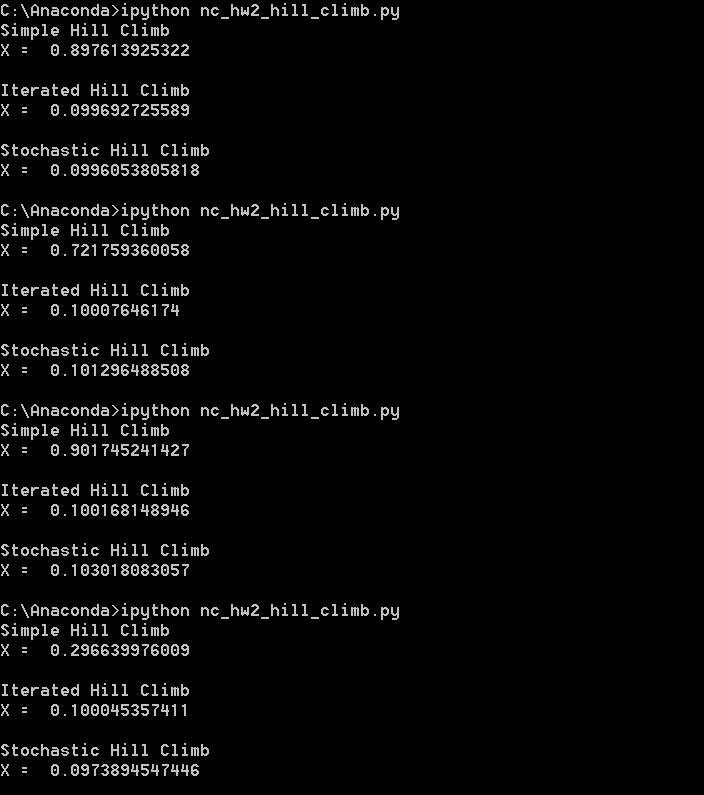
\includegraphics[width=0.75\textwidth]{/HillClimb.PNG}
%\end{center}
%\caption{Sample Hill Climb Algorithms Answers \label{hill_climb} }
%\end{figure}


\newpage
\section{Problem 2}
\textbf{Implement and apply the hill-climbing, simulated annealing, and genetic algorithms to maximize function $g(x)$ used in the previous exercise assuming a bitstring representation.} \newline \\
\textbf{Tip: The pertubation to be introduced in the candidate solutions for the hill-climbing and simulated annealing algorithms may be implemented similarly to the point mutation in genetic algorithms. Note that in this case, no concern is required about the domain of x, because the binary representation already accounts for it.} \newline \\
\textbf{Discuss the performance of the algorithms and asses their sensitivity in relation to the input parameters.}


\newpage
\section{Problem 7}
\textbf{Determine, using genetic programming (GP), the computer program (S-expression) that produces exactly the outputs presented in Table 3.3 for each value of x. The following hypotheses are given:}
\begin{itemize}
\item \textbf{Use only functions with two arguments (binary trees).}
\item \textbf{Largest depth allowed for each tree: 4}
\item \textbf{Function set: F = {+, *}}
\item \textbf{Terminal set: T = {0, 1, 2, 3, 4, 5, x}}
\end{itemize}
\centerline{\begin{tabular}{ c c }
\hline
x & Program output \\
\hline
-10 & 153 \\
\hline
-9 & 120 \\
\hline
-8 & 91 \\
\hline
-7 & 66 \\
\hline
-6 & 45 \\
\hline
-5 & 28 \\
\hline
-4 & 15 \\
\hline
-3 & 6 \\
\hline
-2 & 1 \\
\hline
-1 & 0 \\
\hline
0 & 3 \\
\hline
1 & 10 \\
\hline
2 & 21 \\
\hline
3 & 36 \\
\hline
4 & 55 \\
\hline
5 & 78 \\
\hline
6 & 105 \\
\hline
7 & 136 \\
\hline
8 & 171 \\
\hline
9 & 210 \\
\hline
10 & 253 \\
\hline
\end{tabular}}